% @TODO Change this
\chapter{Background}
\label{chapter2}

The two key concepts we will introduce in this dissertation are the Contour Tree and Persistent Homology. In order to be able to do this we have to first take a step back and walk the reader through a range of other mathematical disciplines. The preliminaries include Point Set Topology, Differential Topology, Algebraic Topology and Graph Theory. We will opt for introducing these fields with a more practical and computational flavour and provide the reader with both the necessary formalism and intuition behind the main definitions and results we will use in the following chapters.

\section{Point Set Topology}

The first branch of Topology that we will introduce is Point Set Topology. It forms the underlying framework on top of which mathematicians build the concepts of continuous spaces and functions. Point Set Topology is the study of sets that posses certain mathematical structure. The core concept in Point Set Topology is the mathematical structure known as the topology of a set. The topology of a set makes the notion of whether two elements of a set are "close" or "near" to one another rigorous. Elements of a set which are close or near to one another are said to be a part of an open set.  In this chapter we will borrow definitions and results from one of the standard introductory topology textbooks \cite{intro-topo}.

\begin{defn} Let $X$ be a set and $\tau$ be a set of subsets of $X$. The set $\tau$ is a topology on $X$ when the following holds:  \end{defn}

\begin{itemize}
    \item $X \text{ and } \emptyset \in \tau$.
    \item If $U \text{ and } V \in \tau$ then $U \cap V \in \tau$.
    \item If $\{U_\lambda\}_{\lambda \in \Lambda}$ is a family of subsets of $X$, where $U_\lambda \in \tau$ for all $\lambda \in \Lambda$, then
        $\bigcup_{\lambda \in \Lambda}{U_\lambda} \in \tau$.
\end{itemize}

We will call the elements of $X$ points and the elements of $\tau$ open sets or simply open. An open set is an open neighbourhood of a point when the point is in the open set. We must stress that the topology we endow on a set is by no means unique. For example if $X$ is any set then one valid topology on $X$ may consist of all subsets of $X$ while another may simply be $\{\emptyset, X\}$.

Let us now introduce the topology we are going to use on n-dimensional Euclidean space or simply $\mathbb{R}^n$. It is called the standard topology and it is based on the standard definition of distance between points in $\mathbb{R}^n$. Let $x = (x_1, x_2, ..., x_n)$ be a point in $\mathbb{R}^n$. We can define the open ball around $x$ of radius $\epsilon$ as $B_\epsilon(x) = \{y \in \mathbb{R}^n: d(x, y) < \epsilon\}$ where we define the distance function as $d(x, y) = \sqrt{\sum_{i=1}^n{(x_i - y_i)^2}}$. The standard topology on $\mathbb{R}^n$ consists of the open balls around all points of all possible radii and their finite intersections and arbitrary unions.

% But how is it possible to update this? How fast is it? * What do you mean by this? *

% @TODO Expand if you have time
Next we will define a special class of functions that preserve the properties of topological spaces. Those are the continuous functions.

\begin{defn} A function $f : X \to Y$ is said to be continuous when the preimage of an open set in $Y$ is an open set in $X$. \end{defn}

In formal notation if $U \in Y$ is open in $Y$ then $f^{-1}(U)$ is open in $X$. This definition captures the understanding we have of continuity from calculus in the more general context of topology. If $f$ is a bijection and $f^{-1}$ is also continuous we will call $f$ a homeomorphism. Homeomorphisms play a special role in topology. Two topological spaces are homeomorphic when there exists a homeomorphism between then. As continuous functions preserve open sets it follows that homeomorphic spaces are topologically identical. This is the reason why topologists are mostly interested in classifying and analysing spaces up to homeomorphism.



% This definition captures the intuitive understanding we have of continuity from calculus - if we "slightly adjust" the output of a function in $Y$ then there should be a "slight change" in input in $X$. The "slight change" is formalised by considering all points in a single open set, as we can think of them as being "near".
%Homeomorphism is the appropriate equivalence relation for topological spaces [].

We will call a property of a space that is preserved under homeomorphisms a topological invariant. The first topological invariant we will introduce is path-connectedness. Path-connectedness is based on paths between points in a topological space.

\begin{defn} Let $X$ be a topological space and let $x, y \in X$ be any two points. A path between $x$ and $y$ in $X$ is a continuous function $f: [0, 1] \to X$ such that $f(0) = x$ and $f(1) = y$.  \end{defn}

% @TODO Add this
Using this definition we can define a path-connected topological space as follows.

\begin{defn} A topological space $X$ is said to be path-connected if there exists a path between any two points $x, y \in X$  \end{defn}

% This definition actually describes  the methodologies for analysing topological spaces. Through defining auxiliary some auxiliary structure. In the case of path-connectedness we have employed a two parameter family of utility functions to "measure" a global property of the topological space - whether it is path connected or not. The two parameter family is the collection of all paths between all pairs of points.

Topological invariants play a crucial role in differentiating between topological spaces. Since path-connectedness is a topological invariant the continuous image of a path-connected topological space is also path-connected.  It follows that there cannot exist a homeomorphism between a topological space that is path-connected and on that is not.

We will now introduce two different ways in which you can obtain new topologies from already known topologies. The first way is known as the subspace topology. A subspace of a topological space $X$ is any subset of points in $X$.

\begin{defn} Let $A \subseteq X$ be a suspace of $X$. Wwe define the open sets for a topology on $A$ as the intersection of the open sets in $X$ with $A$. \end{defn}

This means that a set $U \subseteq A$ is open in $A$ exactly when $U = U' \cap A$ where $U'$ is open in $X$. This result allows us to obtain a topology of $A$ by taking all possible intersections of the open sets in $X$ with $A$. For example let $X = \mathbb{R}$ and $A = [0, 1]$. The set $[0, 1/2) = (-1/2, 1/2) \cap [0, 1]$ is open in $A$ because $(-1/2, 1/2)$ is open in $X$
. This does not imply that $[0, 1/2)$ is open in the topology of $X$, only in the topology of $A$.

The second way of obtaining new topologies is via the quotient topology. To understand it we must first define a quotient space via an equivalence relation. An equivalence relation $\sim$ defined on a topological space $X$ partitions all points in $X$ into equivalence classes. The equivalence class of a point $x \in X$ is the set $[x] = \{y \in X: x \sim y\}$. The set of all equivalence classes is called the quotient of $X$ by $\sim$ and denoted as $X / \sim$. Let also $\pi: X \to X/ \sim$ be the map that takes a point $x$ of $X$ to its equivalence class in $X / \sim$.

\begin{defn} Let $X$ be a topological space and $\sim$ be an equivalence relation defined on $X$. The quotient topology of $X / \sim$ is formed by the sets $U \subseteq X / \sim$ such that $\pi^{-1}(U)$ is open in $X$. \end{defn}

By this definition the function $\pi$ is continuous. We can use this fact to infer that if a topological space $X$ is path-connected then $X / \sim$ is path connected for any equivalence relation $\sim$ because there exists a continuous function $\pi : X \to X / \sim$. An important example is when we take quotients of subsets of topological spaces. Let $A \subseteq X$. We can define an equivalence relation as $x \sim y$ whenever both $x, y \in A$. We will call the resulting quotient space $X / A$. The geometrical interpretation of $X / A$ is that all points in $A$ are contracted to a single point in $X / A$. As a direct example of this consider the closed disk $D = \{x^2 + y^2 \le 1\}$ and its subset the circle $S^1 = \{x^2 + y^2 = 1\}$.
The quotient space $D / S^1$ is homeomorphic to the three dimensional sphere $S^2 = \{x^2 + y^2 + z^2 = 1\}$.

% To see why this is true imagine embedding $D$ in the $xy$ plane of a three dimensional space. Now imagine contracting all points along $S^1$ to a single point above the $xy$ plane. The resulting object resembles $S^2$ but with a cusp.

Now we will present our final definition. That of a topological manifold - a mathematical generalisation of a surface.

% @TODO Should it be an open neighbourhood?
\begin{defn} A $d-manifold$ is topological space where every point has an neighbourhood that is homeomorphic to $\mathbb{R}^d$.  \end{defn}

% @TODO Redo last sentence.
An example of a 0-dimensional manifold is a single point in $\mathbb{R}^n$. Examples of one dimensional manifolds are lines, circles, graphs and curves. Examples of 2-dimensional manifolds are the surfaces we are familiar with from geometry such as the sphere, the torus and so on. In this dissertation we will only consider manifolds of dimension zero, one, two and three. The reason for this is that our primary focus is on the visualisation aspect of computational topology. Visually modelling natural spacial phenomena prohibits us from using high dimensional manifolds they cannot be properly embedded in two or three dimensional Eucledian space.

% *Manifolds are the playground where topology meets geometry.*

% @TODO Redo last sentence. Why?
It is often difficult to analyse the topology of a space by just considering its open sets. This is why in the following two sections we will employ additional tools from other fields of mathematics to aid in our analysis of the topology of a space. These tools are differentiable functions over differentiable spaces and combinatorial approximations of topological spaces.


\section{Differential Topology}

Differential topology is the study of differentiable functions defined on differentiable manifolds. One of the most well developed fields of differential topology is Morse Theory \cite{morse-theory-book, morse-theory-book-milnor}. Morse theory is the study of the relationship between spaces and functions defined on them. One way we can study manifolds via differentiable functions is by analysing the critical values of the functions. Due to complexity of doing so especially in relation to degenerate critical points we will restrict ourself to a special class of differentiable functions called Morse functions.

% One of the main goals is to determine the shape of a space by analysing the class of functions that can be defined on it.

% This however is an enormous task in its own right.
% For example using methods from differential topology we can show that the real line and the circle are different topologically. * See Appendix for example.*

\begin{defn} A function $f: M \to \mathbb{R}^n$ is a Morse Function if $f$ is smooth and at critical points the Hessian (matrix of second partial derivatives) is full rank.   \end{defn}

In order to analyse the topoogy of scalar fields will restrict our attention even further and consider Morse functions whose codomain is $\mathbb{R}$. Points of $M$ whose first derivative is zero are called critical points. All other points of $M$ are called regular.

We can use a Morse function defined on a manifold to decompose it into a family of path-connected subsets. We can analyse the subsets to obtain global topological information about the connectivity of the manifold. Examples of such families of subsets are level sets, sublevel sets and super level sets.

\begin{defn} A level set at a value $h$ of a Morse function $f: M \to \mathbb{R}$ is the set $f^{-1}(\{h\}) = \{x \in M: f(x) = h \}$   \end{defn}

Sublevel sets are defined in terms of the preimage of $f$ of intervals of the form $[-\infty, a]$. A sublevel set at $a$ is defined as $f^{-1}([-\infty, a]) = \{x \in M: f(x) \in [-\infty, a] \}$. Superlevel sets are defined analogously in terms of intervals of the form $[a, \infty]$.
% @TODO Include this somewhere else?
% We will call the path-connected components of a level set contours.

% @TODO Explain Critical Points and Critical Value.

Morse functions ensures the following properties hold:

\begin{itemize}
    \item None of the critical points are degenerate.
    \item Changes in the topology of level sets, sublevel sets and superlevel sets only happen at critical points.
    \item A Morse function defined on a surface has a finite number of critical points.
\end{itemize}

Morse functions allow us to decompose a manifold into its level sets. We will use the theory we have developed so far to introduce the principal tool that allows us to analyse how the connectivity of level sets $f^{-1}(\{h\})$ changes as we vary the input parameter $h$.

\subsection{Reeb Graph}

% @TODO Define the quotient topology. Also I'm not sure if you definition of reeb graph is correct!


The Reeb Graph is a tool that encapsulates the evolution of the topology of level sets of a continuous function. When the function is Morse, an edge in the Reeb graph corresponds to a sequence of contours in the level sets whose topology does not change. The vertices correspond to critical points where the topology of those components does changes. An example of a topological change is when connected components in the level sets appear or dissapear or when two connected components split or merge. Morse theory ensures that critical points occur at distinct values of the parameter and are isolated. This removes ambiguities that may arise in the construction of the Reeb graph.

\begin{defn}
Given a topological space $X$ and a continuous function $f: X \to \mathbb{R}$ we can define an equivalence relation $\sim$ such that two points $x, y$ in $X$ are equivalent when there exists a path between them in a level set $f^{-1}(\{h\})$ for some $h \in \mathbb{R}$. The Reeb Graph is the quotient space $X \big/ \sim$ together with the quotient topology.
\end{defn}

We can think of the Reeb graph of a space $X$ as the quotient space where the connected components of all level sets are contracted to a single point. The resulting topological graph can also be though of as a discrete graph. To do se we must enumerate the vertices and record all edges between them.

The reason we have defined Reeb graphs is because the contour tree is a special case of the Reeb graph. We will leave it as this and return to the topic in the begining of the next chapter. Before doing so we must take a look at certain tools from Algebraic Topology that allows us to translate the continuous mathematical results we have obtained so far into the realm of finite combinatorial structures that would allow us to perform actual computation.

\section{Algebraic Topology}

% @TODO Incorrect English in last sentece
Algebraic Topology is a branch of topology that uses tools from the field of abstract algebra to study topological spaces. The primary goal is to derive algebraic structures such as groups, rings and vector spaces from topological spaces that remain invariant under continuous mappings. Modern Algebraic Topology has its roots in combinatorially defined topological spaces \cite{combinatorial-algebraic-topology}. Unlike Point Set Topology and Differential Topology this allows us to obtain exact algorithms for computing the algebraic invariants we are interested in. To make matters clearer we will introduce one of the most basic combinatorial topological spaces - Simplicial Comlexes and then we will introduce one of the earliest discovered algebraic invariants - the Euler Characteristic. We will continue our discussion on Algebraic Topology in Chapter [] where we will see how the concept of the Euler Characteristic can be generalised to the field of Algebraic Topology called Homology.

\subsection{Simplicial Complexes}

Simplical Complexes are the one of the first combinatorially flavoured topological spaces one encounters in Algebraic Topology. A simplicial complex is a subset of $\mathbb{R}^n$ that consists of points, line segments, triangles and their higher dimensional analogues attached to one another in a single geometric object. In order to understand simplicial complexes we must first define their basic building blocks \cite{comp-topo}.

\begin{defn} Let $\{v_0, ..., v_k\}$ be $k$ points in $\mathbb{R}^n$. The convex combination of the points is the sum $\sum_{i=0}^k{\lambda_iv_i}$ where $\lambda_i \ge 0$ and $\sum_{i=0}^n{\lambda_i} = 1$.  \end{defn}

If we decide to take the subset of $\mathbb{R}^n$ covered by all possible convex combination we obtain the convex hull of the points.

\begin{defn} Let $\{v_0, ..., v_k\}$ be points in $\mathbb{R}^{k+1}$. The convex combination of those points is the $k-simplex$ defined by the points. We will write that simplex as $[v_0, ..., v_n] \subset \mathbb{R}^{k+1}$  \end{defn}

\begin{figure}[h]%
    \centering
    \subfloat[Vertex]{{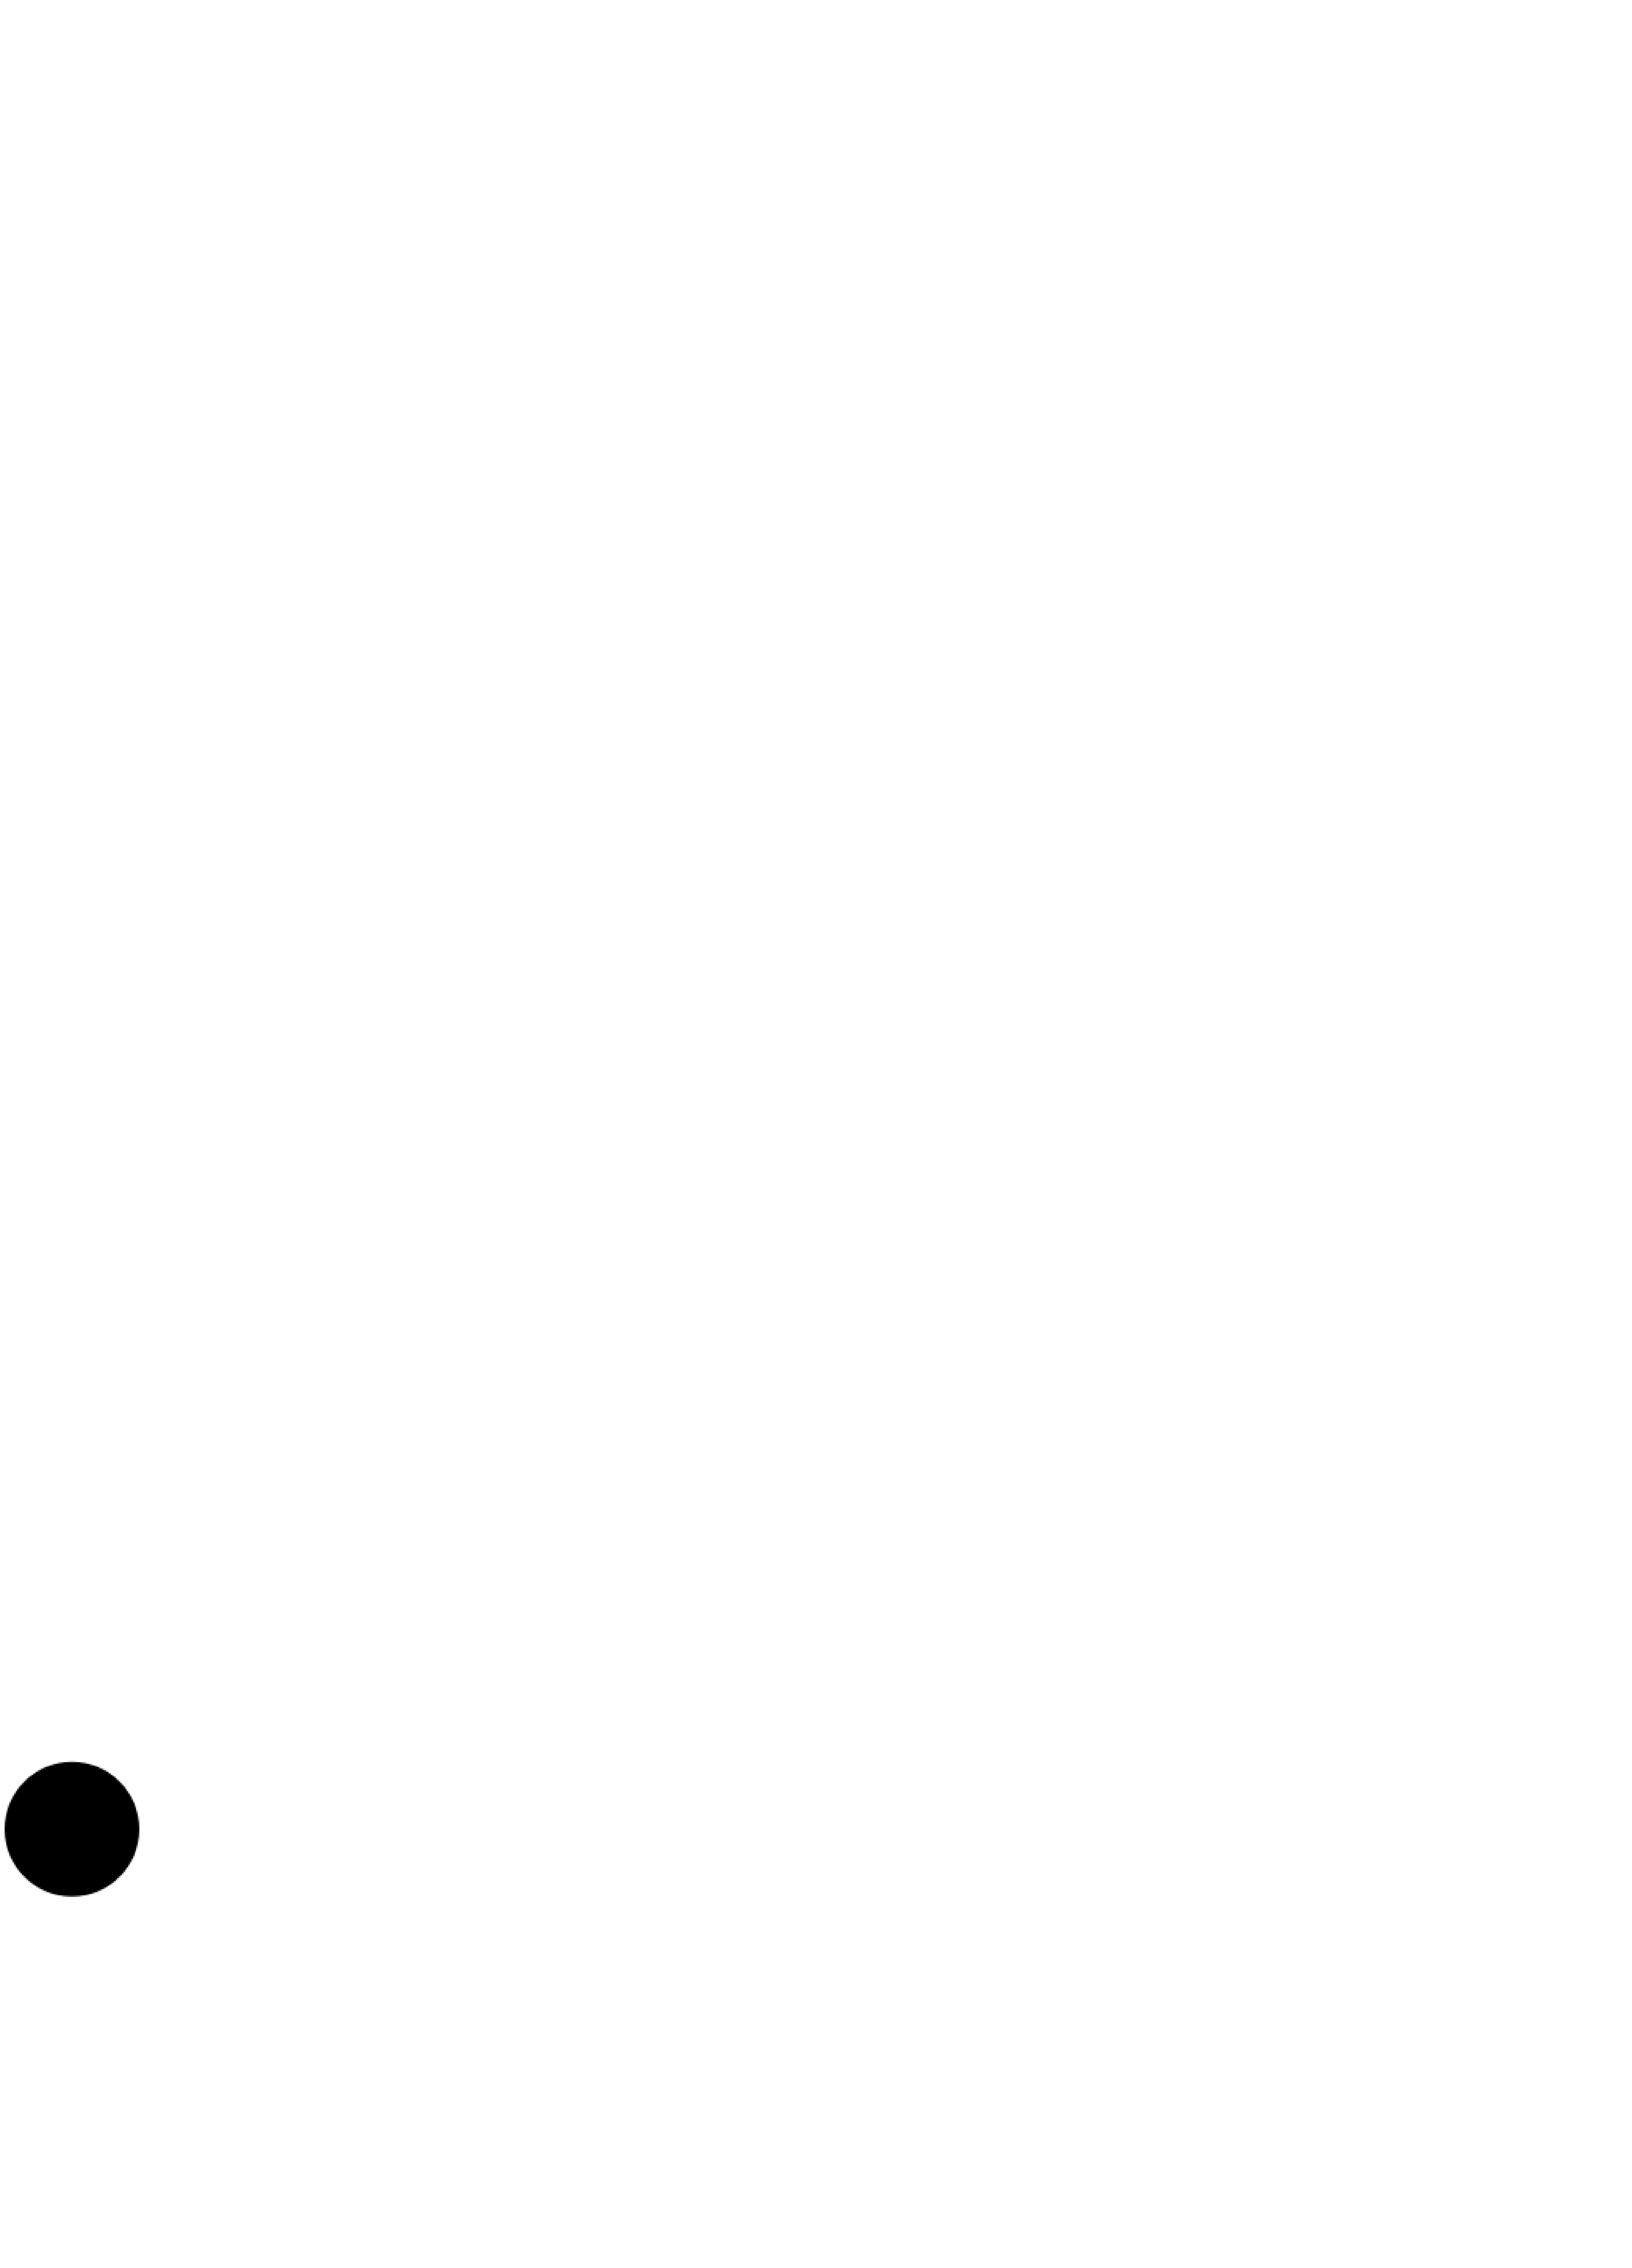
\includegraphics[scale=0.025]{./images/simplex/vertex.eps}}}%
    \subfloat[Edge]{{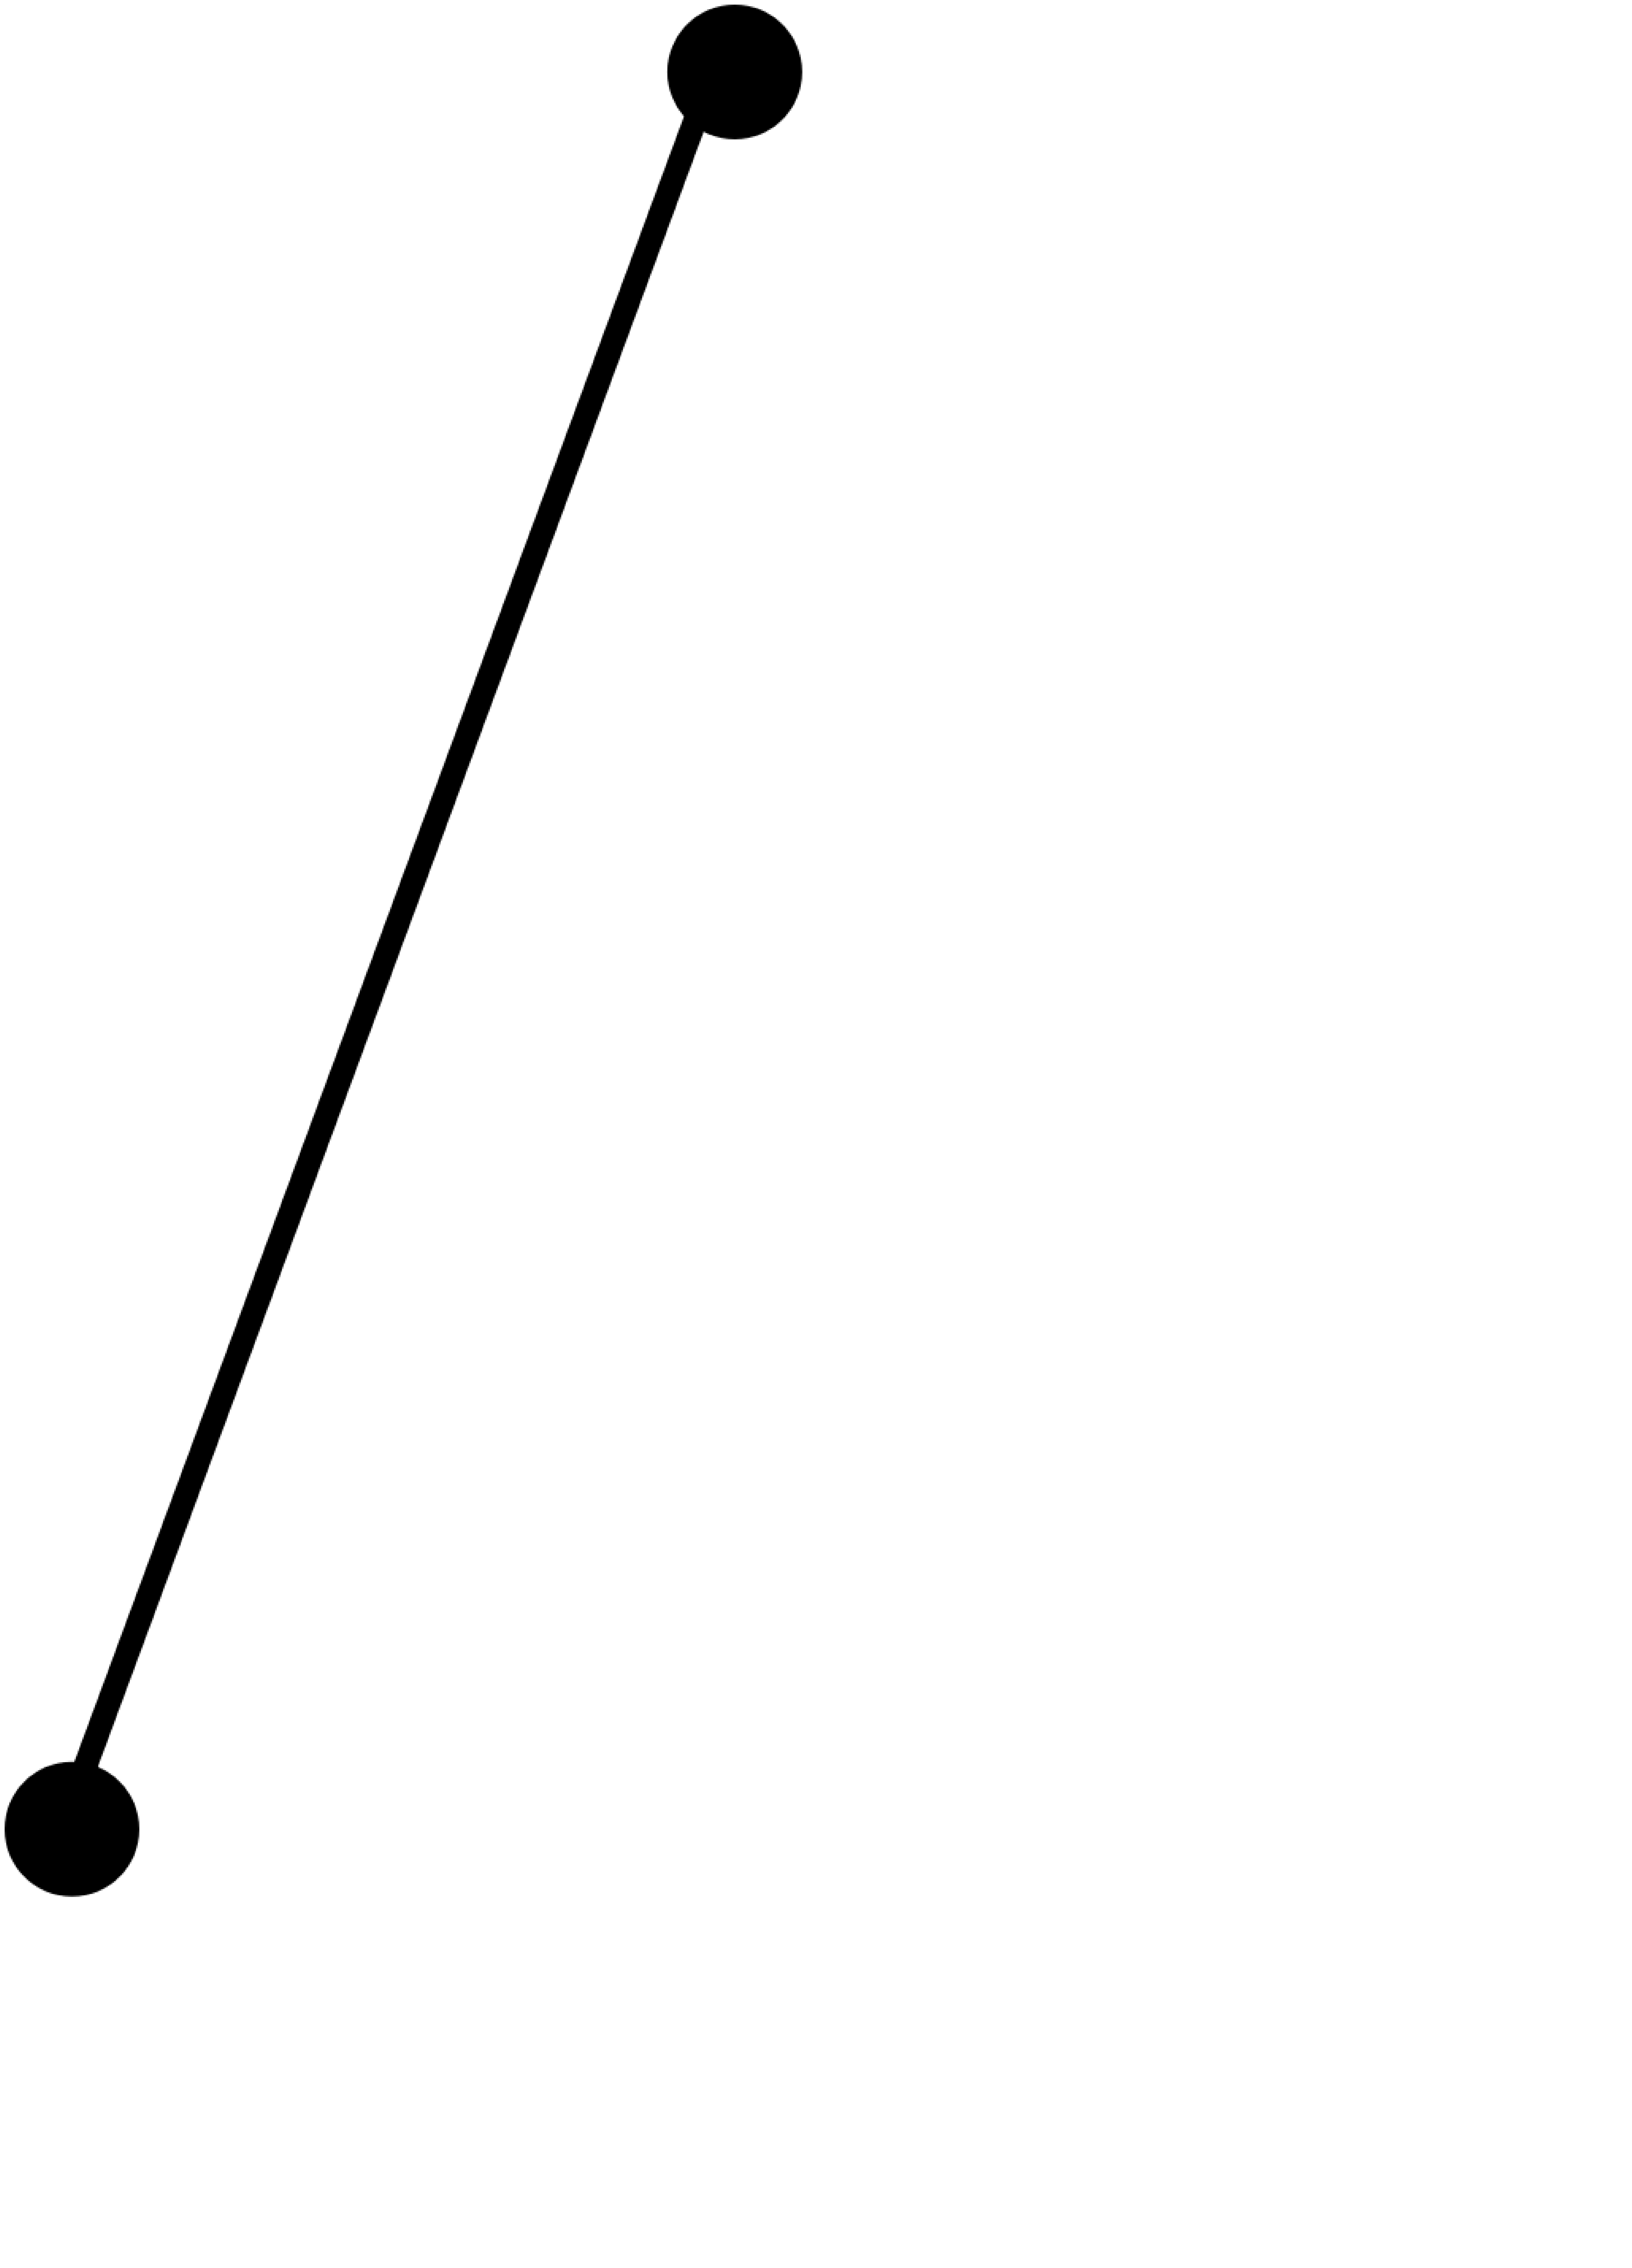
\includegraphics[scale=0.025]{./images/simplex/edge.eps}}}%
    \subfloat[Triangle]{{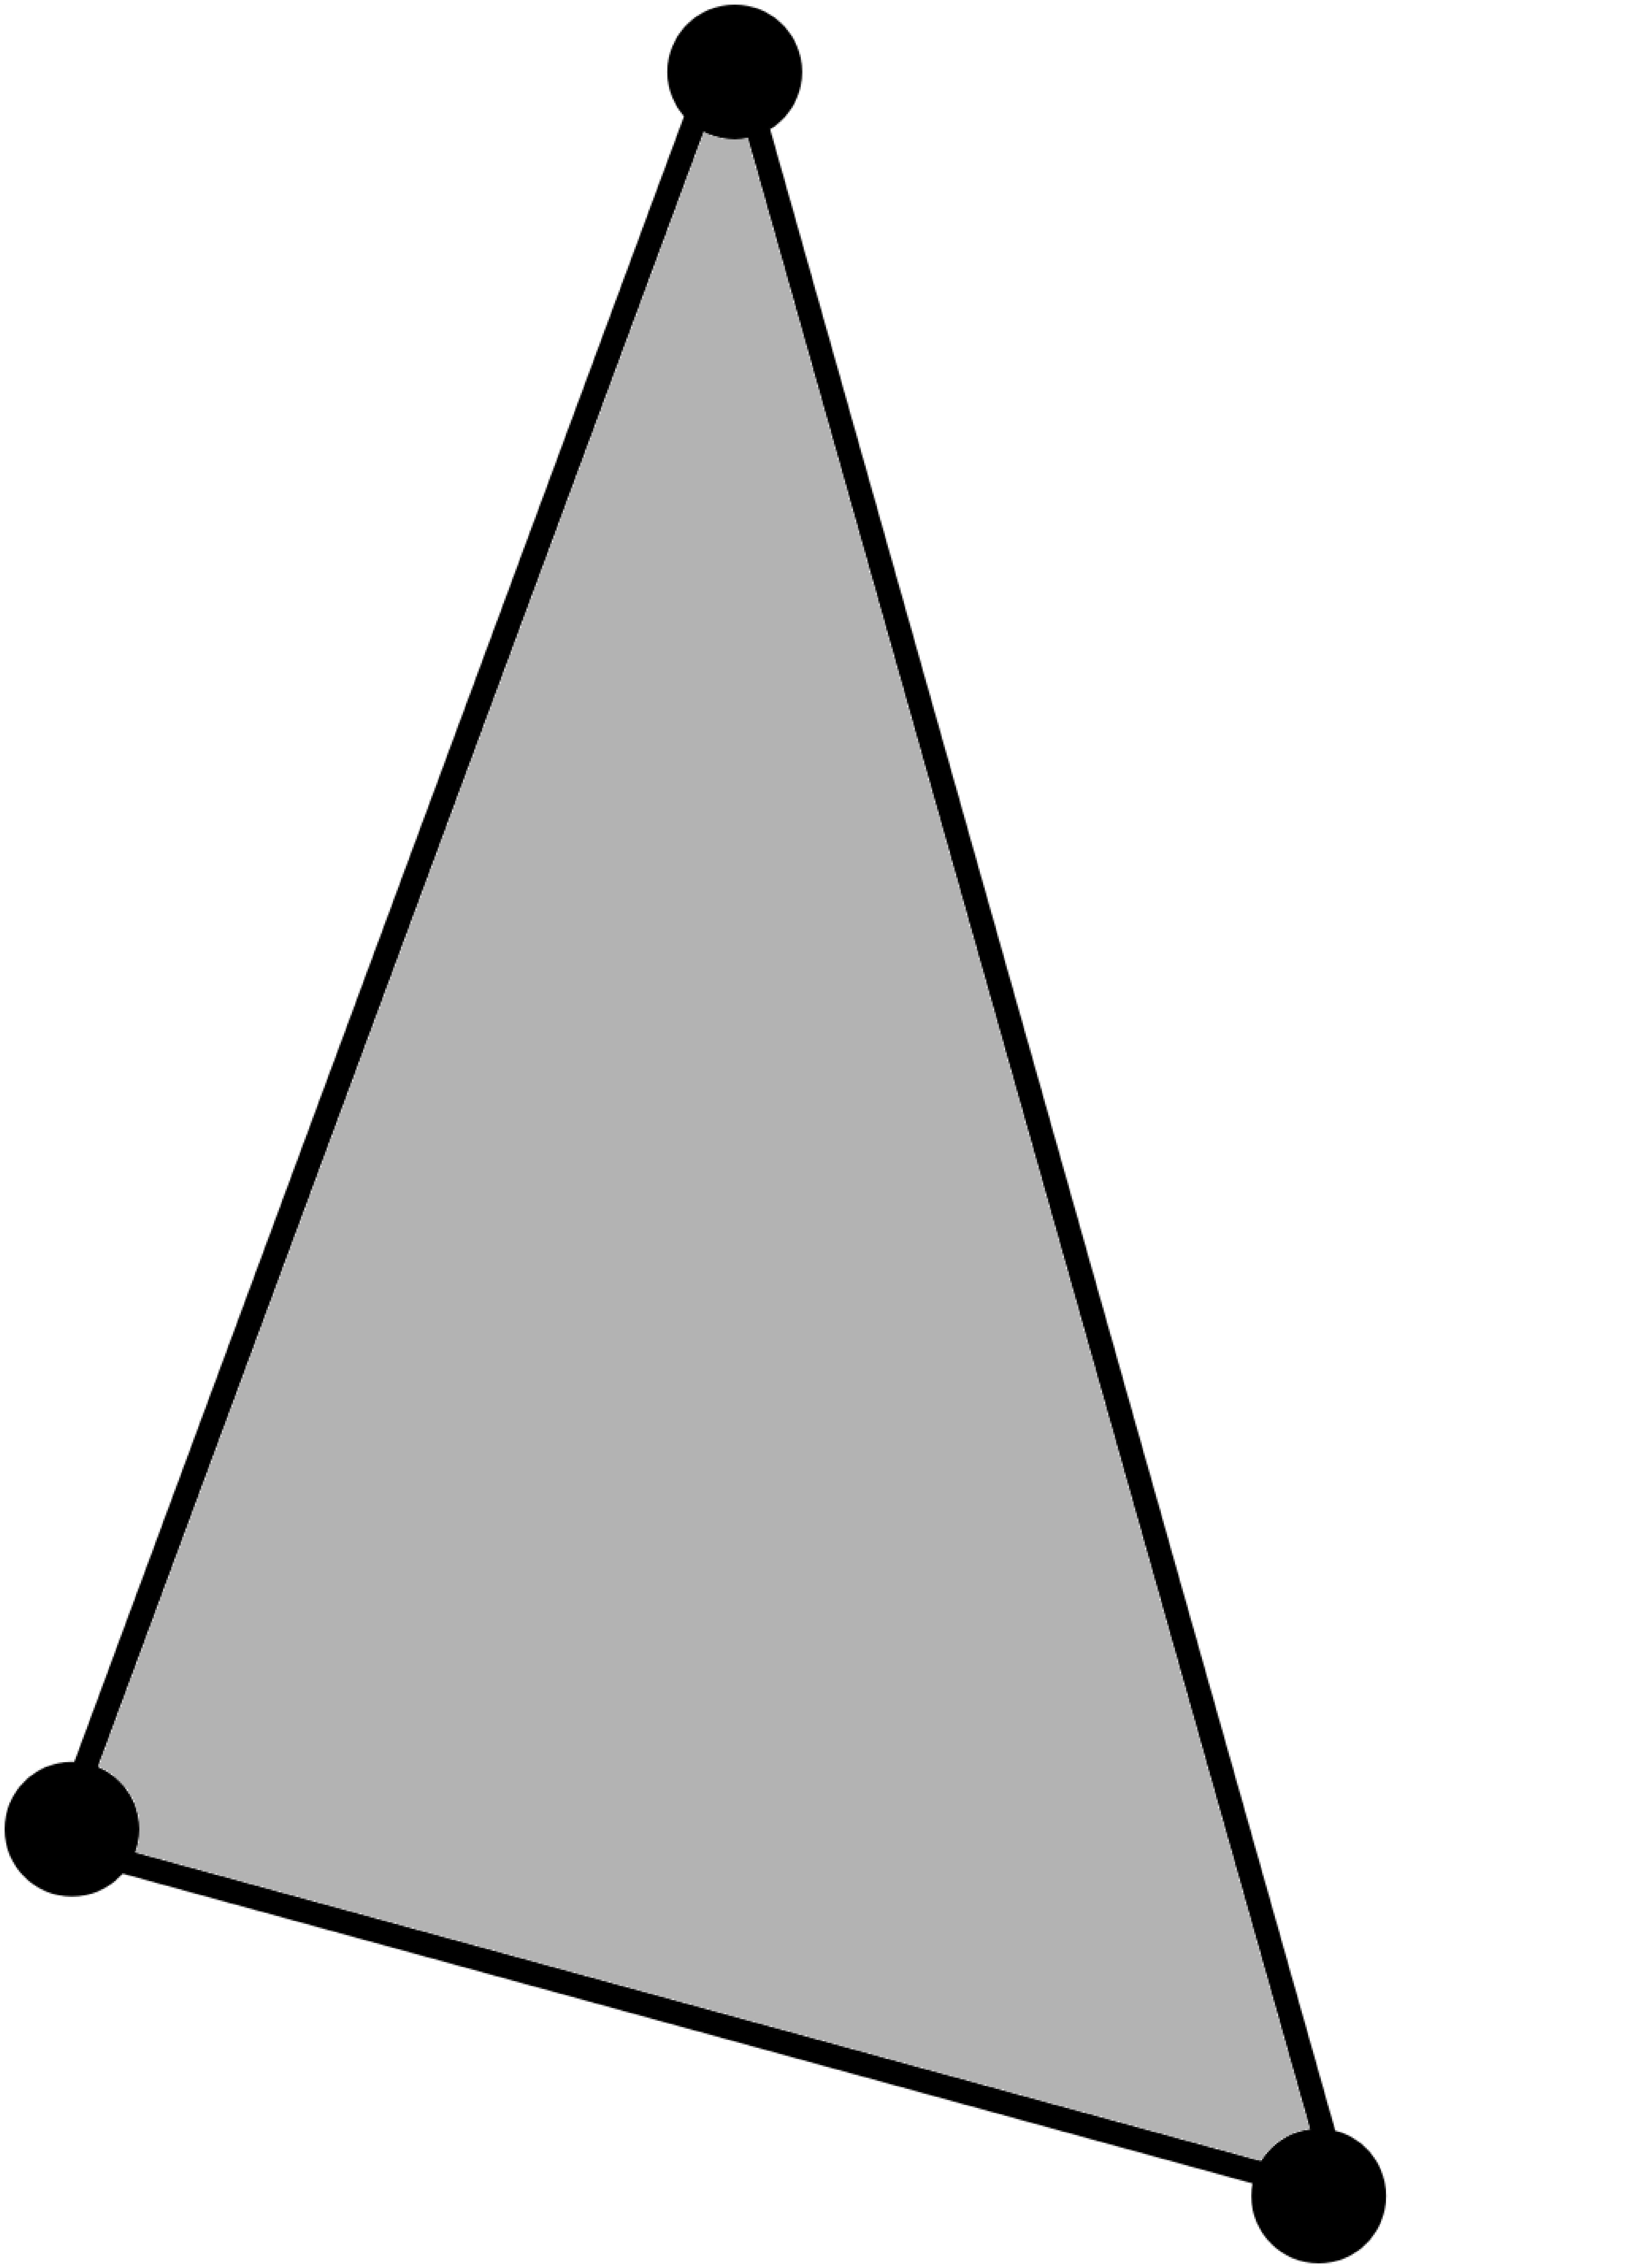
\includegraphics[scale=0.025]{./images/simplex/triangle.eps}}}%
    \subfloat[Tetrahedron]{{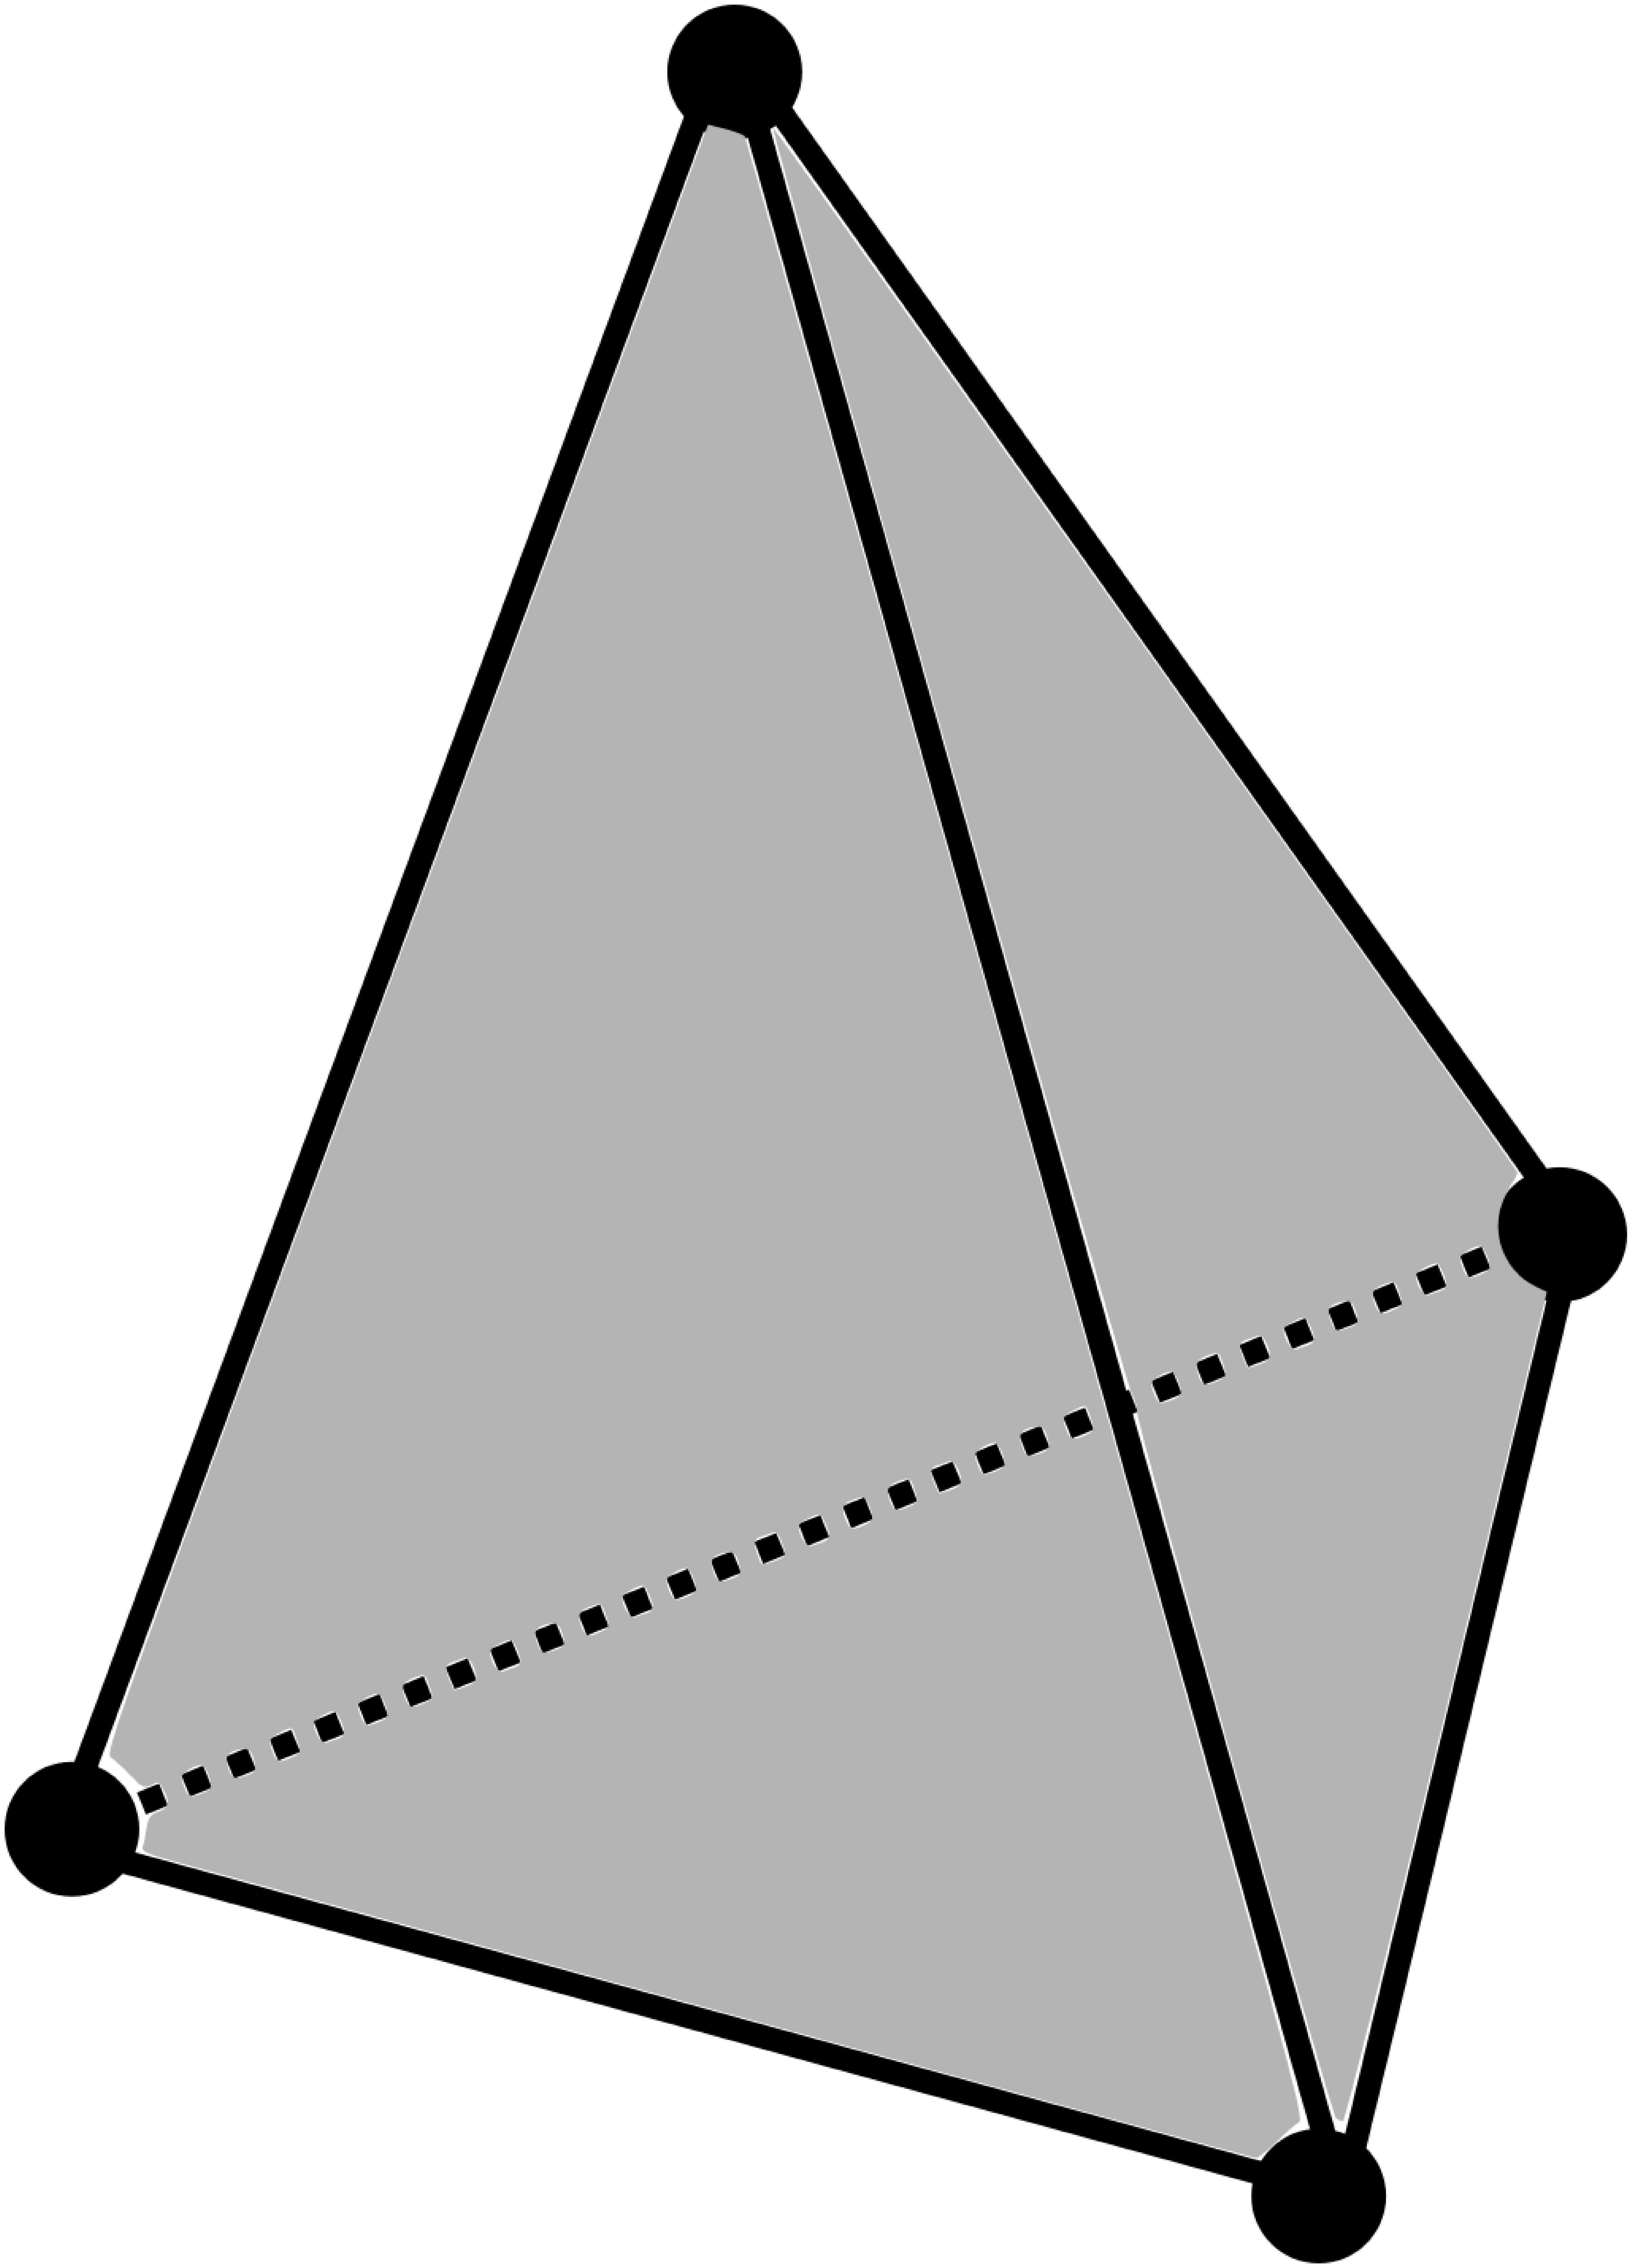
\includegraphics[scale=0.025]{./images/simplex/tet.eps}}}%

    \caption{Simplices of dimension $0, 1, 2$ and $3$.}%
    \label{fig:example}%
\end{figure}

The number $k$ is also called the dimension of the simplex.

We will call the simplices of dimension $0, 1, 2 \text{ and } 3$ vertices, edges, triangles and tetrahedron respectively. As we have mentioned previous we are primarily interested in introducing mathematics as a tool to use in visualisation. Therefore we will have no use for simplices of higher dimension so will avoid naming them altogether.

A face of a simplex is the convex hull of a non-empty subsets of its points. For example the faces of the tetrahedron are the four triangles, six edges and four vertices. To construct a simplical complex all we have to do is take the union of a number of simplices  and "glue" them together along common faces without allowing self-intersection.

\begin{defn} A simplical complex $K$ is a finite collection of simplices such that if $\tau$ is a simplex $K$ then all faces of $\tau$ must be simplicies in $K$. Furthermore the intersection of two simplicies in $K$ is either empty or a common face of both.  \end{defn}


\begin{figure}[h]%
    \centering
    
\includegraphics[center, scale=0.03 ]{./images/simplex/complex.eps}
    \caption{A simplicial comlex.}%
    \label{fig:case1.1}%
\end{figure}


We obtain the topology of a simplicial complex by embedding it in Euclidean space and considering its subspace topology as a subet. After formalising the concept of a simplical complex we will introduce our first algebraic invariant.


\subsection{Euler Characteristic}

The first topological invariant of algebraic nature we shall encounter is the Euler Characteristic. It is denoted as $\chi$ and it assigns an integer to simplical complexes through a generalisation of counting \cite{elementary-applied-topology}. The concept was originally defined for polyhedra as an alternating sum of the form $|V| - |E| + |F|$, where $V$ is the set of vertices, $E$ the set of edges and $F$ the set of faces. The Euler Characteristic can be generalized to simplical complexes as as a infinite alternating sum 3-dimensional simplices, 4-dimensional simplices and so on.

% continue it indefinitely with the number of 3-cells, then 4-cells, etc., as follows
%
%
% % For example this allowed for the classification of the Platonic solids [].
%
% % @TODO Define CW complexes, simplical complexes may not generalise polyhedra
%
%
% all spaces that can be decomposed into a finite number of cells. Let us first consider simplical complexes *because they generalise polyhedra*. The natural generalisation of the alternating sum is to continue it indefinitely with the number of 3-cells, then 4-cells, etc., as follows

$$ \chi = k_0 - k_1 + k_2 - ... = \sum_{i}{(-1)^i~k_i}, $$

where all $k_i$ is the number of $i$-dimensional simplicies for $i \in \mathbb{Z}^+$ and $k_j = 0$ for $i$ bigger than the dimension of the highest dimensional simplex in the simplicial complex.

The Euler Characteristic is a topological invariant. This allows us to compute the Euler Characteristic of topological spaces which are not simplicial complexes. Let us take for example the sphere. We will call any simplicial complex that is homeomorphic to the sphere its triangulation. The most basic triangulation of the sphere is the tetrahedron (excluding its volume). Therefore the Euler Characteristic of the sphere is $\chi = 4 - 6 + 4 = 2$.
% We will use a similar process to compute the contour tree in the next chapter. We will start with an assumption that we have a bounded volume in $\mathbb{R}^2$ and we will triangulate it to enable computation.

\section{Graph Theory}

The last piece of background theory we will cover is from Graph Theory. In this disertation we will make use of certain notation and algorithms that we will define here.

\subsection{General Graph Theory}

We will assume that the reader has is familiar with basic concepts from graph theory such as graphs, subgraphs, vertices, edges, paths and cycles and the basic algorithm such as Breadth First Search (BFS) and Depth First Search (DFS) \cite{intro-to-algo}. For a graph $G = (V, E)$ we will use notation $V(G)$ for the vertices of $G$ and $E(G)$ for the edges of $G$. We will use the notation $N(u)$ for the neighbouhood of $u$ or all the vertices $u$ is adjacent to. We will the notation $d(u, v)$ wherer $u, v \in V(G)$ for the length of the shortes path between $u$ and $v$ in $G$.

Throughout this dissertation most of the graphs we will be working with will be trees. A tree is a connected graph that has no cycles. We will typically refer to trees as $T = (V, E)$. For our intents and purposes we shall define a subtree of a tree as a connected subgraph of a tree. We will refer to subtrees of rooted trees by their root. If $T$ is a rooted tree and $u$ is a node in $T$ then $T_u$ is the subtree of $T$ whoose root is $u$. In this notation if $s$ is the root of $T$ then $T_s = T$. If $u$ is any vertex that is not the root of $T$ then $T_u$ is the (vertex-wise) maximal subtree of $T$ that contains $u$ but does not contain the parent of $u$.

% The height of a rooted tree $T$ is defined as the longest path that starts at the root of the tree. The height of a rooted subtree $T_u$ of $T$ is simply the height of $T_u$ as a rooted tree.

In Chapter [] we will be interested in finding the longest path in a tree. This is known as the diameter of a tree. Here we will  describe two of the most well known linear time tree diameter algorithms.

\subsection{Tree Diameter Algorithms}

The first algorithm we will discuss is based on the following theoretical result [].

\begin{lem} \label{2xbfs-lemma} Let $s$ be any vertex in a tree. The most distant vertex from $s$ is an endpoint of a tree diameter. \end{lem}

To implement this algorithm we require a way of finding the most distant vertex from a given vertex. This can be done using Breadth First Search (BFS). Let $T$ be a tree and $s \in V(T)$ be any vertex. We can run BFS with $s$ as its root to find a vertex $u$ such that $d(s, u) \ge d(s, t)$ for all $t \in V(T)$. We can then run a second BFS with root $u$ to obtain a vertex $v$ such that $d(u, v) \ge d(u, t)$ for all $t \in V(T)$. Since $u$ is the farthest vertex from $s$ by Lemma~\ref{2xbfs-lemma} it must be the endpoint of a diameter. The diameter of $T$ is the longest path in $T$. Therefore the second BSF produces a path whose length as much as the diameter of $T$. Therefore $d(u, v) \ge d(a, b)$ for all $a,b \in V(T)$.

The space and time complexity of BSF are linear \cite{intro-to-algo} and therefore the space and time complexity of this algorithm are linear as well. This follows from that fact that the algorithm consists of running BFS two consecutive times.

The second approach is based on the Dynamic Programming paradigm. Dynamic programming is a method that is used to solve optimisation problems whose solution can be refomulated recursively through solutions of subproblems of the original problem. The key ingredients in developing a dynamic programming algorithm are \cite{intro-to-algo}:

\begin{enumerate}
    \item Characterise the structure of the optimal solution.
    \item Recursively define the value of the optimal solution.
    \item Compute the value of the optimal solution.
\end{enumerate}

% @TODO Redefine N(u)

We will characterise the structure of the optimal solution through all subtrees of a tree. If we root a tree $T$ in any of its vertices then then structure of the optimal solution is defined via all the rooted subtrees of $T$ or $\{T_u\}_{u \in V(G)}$. We can recursively define the value of the optimal solution with the following observation. Starting at the root, of the tree the longest path in the tree either goes through the root or is entirely contained in one of the subtrees rooted at the children of the root. This reasoning can be extended to all rooted subtrees of the tree.

In order to formalise this idea we will make use of two functions. Let $T$ be a rooted tree with root $s$. Let $h(u)$ be the height of the subtree rooted at $u$. The height is defined as the longest path in $T_u$ from $u$ to one of the leaves of $T_u$. We will also call such a path a height path. Let $D(u)$ be the length of the longest path contained entirely in $T_u$. The function $D$ will contain the value of the optimal solution for all subtrees. The value of $D(s)$ is either equal to the value of $D(u)$ where $u$ is a child of $s$ or it is equal to combining the two maximum height paths of two of the children of $u$. This is sumamrised by he following formula.

$$ D(s) = max\bigg\{ \max\limits_{u \in N(s)}\bigg(D(u)\bigg), \max\limits_{\substack{u, v \in N(s) \\ u \ne v}} \bigg(h(u) + h(v) + 2\bigg) , \max\limits_{u \in N(s)}\bigg(h(u) + 1 \bigg)   \bigg\}. $$

The first terms describes the case when the longest path is contained entirely in one of the subtrees rooted at a child of $s$. The second terms combines the two longest height paths in two distinct children $u, v$ of $s$ and adds an aditional $2$ to account for the edges $us$ and $vs$. The last term is given in the case where $s$ has exactly on child and we cannot combine two height paths.

The base case for this recursive formula is at the leaves of $T$. If $u$ is a leaf of $T$ then $V(T_u) = \{u\}$. This allows us to set $h(u) = 0$ and $D(u) = 0$ and consider all leaves as base cases for the recursive formula. This algorithm can be implemented in linear time using Depth First Search (DFS) by using two auxiliary arrays that hold the values for $h(u)$ and $D(u)$ for every $u \in V(T)$. For the implementational details we refer the reader to [].

% We will elaborate more on the imeplementational details in the final section of this chapter.

% We are guaranteed to reach the base cases because all subtrees in the formula are strictly smaller.
%
% as each subtree is strictly smaller we must inevitably reach all leaves.

%@TODO Fix sentece before

%This results allows to compute in practice $\chi$ of manifolds by considering any of their finite triangulations. As long as there is a homeomorphism between a manifold and triangulation $\chi$ will not change. We will be well advised to pick the triangulations with the least number of simplices to improve computational efficiency. For example the octahedron is a triangulation of a sphere and therefore the Euler Characteristic of the sphere is zero. For further information on this subject we refer the reader to [].
